\documentclass[10.5pt,a4paper]{article}
\usepackage[margin=2.2cm,headheight=14pt]{geometry}
\usepackage{fontspec,unicode-math}
\setmainfont{Libertinus Serif}\setsansfont{IBM Plex Sans}\setmonofont[Scale=0.84]{IBM Plex Mono}\setmathfont{Libertinus Math}
\usepackage{microtype,graphicx,booktabs,tabularx,xcolor,fvextra,caption,fancyhdr,titlesec,enumitem,amsmath,amsthm,array,placeins,tikz}
\usepackage[colorlinks,linkcolor=teal!60!black,urlcolor=teal!60!black,citecolor=teal!60!black]{hyperref}
\usetikzlibrary{arrows.meta,positioning}
\captionsetup{font=small,labelfont=bf}
\renewcommand{\tabularxcolumn}[1]{>{\raggedright\arraybackslash}p{#1}}
\setlength{\emergencystretch}{3em}\setlist{itemsep=2pt,topsep=3pt}
\titleformat{\section}{\sffamily\Large\bfseries\color{teal!50!black}}{\thesection}{0.8em}{}
\titleformat{\subsection}{\sffamily\large\bfseries}{\thesubsection}{0.7em}{}
\titleformat{\paragraph}[runin]{\sffamily\bfseries}{}{}{}[.]
\newtheorem{theorem}{Theorem}
\pagestyle{fancy}\fancyhf{}\fancyhead[L]{\sffamily\footnotesize AICOR Cell 01: vision, status and demonstrator plan}
\fancyhead[R]{\sffamily\footnotesize\nouppercase{\leftmark}}\fancyfoot[C]{\sffamily\footnotesize\thepage}
\renewcommand{\headrulewidth}{0.3pt}
\renewcommand{\floatpagefraction}{0.7}\renewcommand{\topfraction}{0.9}\renewcommand{\textfraction}{0.1}
\begin{document}
\begin{titlepage}\sffamily
\noindent\includegraphics[width=\linewidth,height=0.42\textheight,keepaspectratio]{/home/mbeetz/Documents/LabAutomationTwin/renders/lab/lab_cell_interior.png}\par\vspace{0.8cm}
{\color{teal!50!black}\rule{\linewidth}{1.2pt}}\par\vspace{0.4cm}
{\Huge\bfseries A laboratory that knows\\[4pt] what its experiments mean\par}\vspace{0.3cm}
{\Large AICOR Cell 01: vision, research problem, contributions,\\ where we are, and the plan for a first demonstrator\par}\vspace{0.3cm}
{\color{teal!50!black}\rule{\linewidth}{1.2pt}}\par\vspace{0.6cm}
{\large Semantic digital twin of an automated culture-experimentation cell\par}\vspace{0.3cm}
{\normalsize [Authors and affiliations] \hfill 18 October 2026\par}\vfill
{\small\rmfamily Every figure, excerpt and number in this document is generated from the LabAutomationTwin repository
(renders from Isaac Sim 6.2, ontologies reasoned by HermiT and Konclude, plans checked by z3). Biology, doses and
timings are Cell 01's illustrative surrogate (decision D016); they are not laboratory facts.\par}
\end{titlepage}
\tableofcontents\clearpage


\section*{Summary}\addcontentsline{toc}{section}{Summary}
Robots in biomedical laboratories execute protocols. They do not know what the experiment is for, which culture is
the control, which comparison answers the question, or whether a failure at 3~am invalidates a conclusion. Cell~01 is
our answer: an automated culture-experimentation cell, built first as a \emph{semantic digital twin}, in which the
experiment itself is represented, reasoned about and executed down to the robot motions, with proofs that the motions
implement the design.

\paragraph{Where we are} The twin is complete: 5 end-to-end robot episodes run in physics
(nominal, identity swap, quarantine and release, imaging, full cell), 110/110 device and robot
acceptance tests pass, and AICOR Lab~1 surrounds the cell. Above it sits a stack of knowledge: a lab designator language
(LDL) that states what lab actions must achieve, an OWL~2~DL experiment ontology (174 concepts, 246 axioms) whose reasoner classifies a design as adequately controlled or not, a 413-concept lab ontology within the AICOR federation, capability profiles that decide what the lab can run,
Bayesian experiment design, and a robot science assistant kernel. A refinement theorem, discharged by machine checks,
states that the 111 robot motions of the selected experiment either realize the culture-level
design under all constraints or stop in a handler whose guarantee holds.

\paragraph{What is next} A first demonstrator: the challenge--rescue experiment executed end to end in the twin by the
generated plans, its cultures imaged by the robot's own camera, the belief updated, faults injected and handled at
the level of the experiment, the improved five-arm design carried through the same proof, and one segment on real
hardware (Section~\ref{sec:plan}).


\section{Vision and mission}
\paragraph{Vision} A laboratory in which a robot scientist runs biomedical experiments that are valid by
construction: every robot action traces to the scientific purpose it serves, every design is checked for the controls
and comparisons its conclusion needs before anything is pipetted, every failure is understood in terms of what it
does to the experiment, and every result carries the evidence of how it was obtained.

\paragraph{Mission} To build Cell~01, an automated cell for culture experiments, as the place where this is worked
out end to end: a physically faithful, semantically annotated digital twin first, with the knowledge, reasoning and
plans that make its robots understand the experiments they perform; then a demonstrator; then real hardware.

\begin{figure}[htbp]\centering\includegraphics[width=\linewidth,height=0.36\textheight,keepaspectratio]{/home/mbeetz/Documents/LabAutomationTwin/renders/lab/lab_overview.png}\caption{AICOR Lab~1 with Cell~01 at its centre (path-traced in Isaac Sim 6.2): operator desks, prep bench, storage, the enclosed cell with its AMR portal.}\end{figure}


\section{The research problem}
\textbf{How can a robot execute a biomedical experiment so that what it physically does provably implements what the
experiment is designed to establish, and so that it knows, at every moment, what its actions, observations and failures
mean for the experiment's conclusions?}

The problem has three parts:
\begin{enumerate}
\item \textbf{Meaning across levels.} An experiment is stated over cultures, treatments, controls and comparisons. A
robot executes motions over plates, grippers and frames. The robot must carry the experiment's meaning down through
these levels and back up: from ``the comparator culture receives the challenge at 0~h'' to 52 grounded steps in one
trip, and from an image of a well back to evidence about a hypothesis.
\item \textbf{Validity, not only execution.} A protocol can run perfectly and still answer nothing: no vehicle control,
no replicates, a confounded comparison, an unvalidated readout. The robot must judge a design's adequacy before running
it, and an execution's validity after.
\item \textbf{Living material under uncertainty.} Cultures change while the robot works; they tolerate only limited
time outside the incubator; their state is seen only through images that are proxies for viability; contamination and
identity swaps happen. Execution must keep the material's constraints and reason about what it does not observe.
\end{enumerate}

\section{Why it matters}
\begin{itemize}
\item \textbf{AI scientists now choose experiments, but nothing checks them.} Agent systems propose and run
experiments on liquid-handling robots~\cite{verid}; their checks concern the protocol and the machine (deck state, safe
commands), not whether the experiment has the controls and comparisons its conclusion needs.
\item \textbf{The syntax-to-safety gap.} Commands that parse can be physically unsafe~\cite{safesdl}; in biology they
can also be scientifically void.
\item \textbf{Reproducibility.} Much of biomedical research does not reproduce~\cite{baker2016}; reporting checklists
are applied by people after the fact.
\item \textbf{Standards stop at devices and data.} SiLA~2, OPC~UA LADS and Allotrope make instruments interoperable and
data contextual~\cite{lapp}; none represents why a step exists or whether a design can answer its question.
\item \textbf{Regulated laboratories need traceability.} Every robot action must be verifiable and auditable, as
TraceBot set out for sterility testing~\cite{tracebot}.
\end{itemize}

\section{Why it is hard}

\begin{table}[htbp]\centering\footnotesize\caption{Why the problem is hard.}
\begin{tabularx}{\linewidth}{@{}p{4.2cm}X@{}}\toprule difficulty & what it means in Cell 01 \\\midrule
The abstraction gap & 12 culture actions become 151 grounded steps in 3 trips and 111 robot motions; each level has its own vocabulary, constraints and failure modes. \\
Time-critical living material & a plate may be outside the incubator for 600~s per excursion (illustrative); culture times (0, 48, 72~h) are fixed by the design. \\
Partial observability & viability is seen through bright-field images of organoid size, core density and debris; the robot's belief must be calibrated against what it cannot see. \\
Validity is not execution & a run can be physically perfect and scientifically invalid (an unvalidated imager: realized but not valid evidence). \\
Failures with consequences & a dropped tip before aspiration is repairable; a misregistered well after the dispense is not; recovery must state what it guarantees. \\
Devices have inner processes & incubators, liquid handlers and imagers have phases, irreversible points and faults that decide how trustworthy a result is. \\
Verification across levels & a proof that motions implement a design must compose discrete planning, continuous control, device contracts and biology. \\
Generality & special devices make automation rigid; general manipulation makes it flexible but harder to verify. \\\bottomrule\end{tabularx}\end{table}


\section{Contributions}
\begin{enumerate}[label=\textbf{C\arabic*}]
\item \textbf{A semantic digital twin of Cell~01 and AICOR Lab~1} (Isaac Sim 6.2): articulated, physically simulated
stations and robots with their own controllers, sensors and monitors, the fit-out, the lab and its site;
5 end-to-end episodes; 110/110 acceptance tests.
\item \textbf{A culture digital twin with two separated worlds}: hidden simulated biology and the robot's belief about
it, connected only by robot records and images; dose ledger, contamination rule, calibrated observation model.
\item \textbf{LDL, a lab designator language}: actions as contracts (requires, prevents, maintains, achieves, goal)
over lab entities only, with instrument roles, device process models, failure handlers with guarantees and an
epistemic meta model; a checked abstraction boundary to the realization.
\item \textbf{The experiment as a reasoned entity}: an OWL~2~DL experiment ontology (174 concepts, 246 axioms) in which HermiT classifies a design by its content: adequately controlled, factorial, interaction-aware;
closed-world checks for what OWL cannot express.
\item \textbf{A lab ontology in the AICOR federation} (413 concepts in 13 modules), bridged to the experiment ontology; the union is consistent and the reasoner proves their arm classes equal.
\item \textbf{Lab affordance}: capability profiles derived from device records, matched against the requirement
classes of designs: what the lab can run, where steps must go, what is missing.
\item \textbf{From information gain to motion}: Bayesian experiment design selects the experiment; an answer-set
program derives the plan; z3 independently validates executability, safety, timing and realization.
\item \textbf{A robot science assistant kernel and CRAM/RPL plans}: designators, executive with failure handling,
two-column critic (realization vs validity), hash-chained audit trail, competency questions; plans generated as
CRAM/RPL and as Giskard motion statecharts.
\item \textbf{A refinement theorem with machine-checked obligations}: the motions implement the culture-level design
or stop in a guaranteed handler, relative to six explicit assumptions; 8 negative controls.
\end{enumerate}


\section{Where we are}
\subsection{The cell and the lab}
Cell~01 combines a fixed plate arm (R01, Franka FR3), a rail-mounted flexible arm with an automatic tool changer
(R02, UR5e), a clean-sample AMR with a deterministic dock (R03/H2), a plate hotel (L09), a CO$_2$ incubator (L10),
a liquid handler (L12), a bright-field imager (L17), a QC and calibration station (L21) and a quarantine station (H4),
inside an interlocked safety enclosure.

\begin{figure}[htbp]\centering\begin{minipage}[t]{0.490\linewidth}\centering\includegraphics[width=\linewidth,height=0.24\textheight,keepaspectratio]{/home/mbeetz/Documents/LabAutomationTwin/renders/lab/lab_cell_front.png}\\[-1pt]{\scriptsize the enclosed cell}\end{minipage}\hfill\begin{minipage}[t]{0.490\linewidth}\centering\includegraphics[width=\linewidth,height=0.24\textheight,keepaspectratio]{/home/mbeetz/Documents/LabAutomationTwin/renders/cell01/cell01_elevated.png}\\[-1pt]{\scriptsize the stations without the enclosure}\end{minipage}\caption{Cell~01 with and without its fit-out (path-traced).}\end{figure}

\begin{figure}[htbp]\centering\begin{minipage}[t]{0.327\linewidth}\centering\includegraphics[width=\linewidth,height=0.17\textheight,keepaspectratio]{/home/mbeetz/Documents/LabAutomationTwin/renders/lab/lab_amr_portal.png}\\[-1pt]{\scriptsize AMR portal}\end{minipage}\hfill\begin{minipage}[t]{0.327\linewidth}\centering\includegraphics[width=\linewidth,height=0.17\textheight,keepaspectratio]{/home/mbeetz/Documents/LabAutomationTwin/renders/lab/lab_storage_dock.png}\\[-1pt]{\scriptsize storage and dock}\end{minipage}\hfill\begin{minipage}[t]{0.327\linewidth}\centering\includegraphics[width=\linewidth,height=0.17\textheight,keepaspectratio]{/home/mbeetz/Documents/LabAutomationTwin/renders/cell01/cell01_r02_magazine.png}\\[-1pt]{\scriptsize R02 and its tool magazine}\end{minipage}\caption{Details of the twin: the AMR route into the cell, storage, and the flexible arm.}\end{figure}


\subsection{Devices and their mechanisms}
Every station is an articulated model whose controller drives its joints in physics and whose sensors feed its
monitors: the L09 hotel's lift, fork and shuttle; the L10 incubator's cassette, lift, gate and environment probes; the
L12 gantry; the L17 stage, focus and turret; the H4 door, latch and shuttle.

\begin{figure}[htbp]\centering\begin{minipage}[t]{0.327\linewidth}\centering\includegraphics[width=\linewidth,height=0.2\textheight,keepaspectratio]{/home/mbeetz/Documents/LabAutomationTwin/renders/l09/l09_cutaway_handler.png}\\[-1pt]{\scriptsize L09: fork carrying a plate}\end{minipage}\hfill\begin{minipage}[t]{0.327\linewidth}\centering\includegraphics[width=\linewidth,height=0.2\textheight,keepaspectratio]{/home/mbeetz/Documents/LabAutomationTwin/renders/devices/l17_open_front_left.png}\\[-1pt]{\scriptsize L17: stage, focus, illumination}\end{minipage}\hfill\begin{minipage}[t]{0.327\linewidth}\centering\includegraphics[width=\linewidth,height=0.2\textheight,keepaspectratio]{/home/mbeetz/Documents/LabAutomationTwin/renders/devices/l10_open_front_left.png}\\[-1pt]{\scriptsize L10: cassette, lift, shuttle}\end{minipage}\caption{Inside the devices (housings removed): the mechanisms the controllers drive.}\end{figure}

\begin{figure}[htbp]\centering\begin{minipage}[t]{0.327\linewidth}\centering\includegraphics[width=\linewidth,height=0.17\textheight,keepaspectratio]{/home/mbeetz/Documents/LabAutomationTwin/renders/devices/l12_front_left.png}\\[-1pt]{\scriptsize L12 gantry and deck}\end{minipage}\hfill\begin{minipage}[t]{0.327\linewidth}\centering\includegraphics[width=\linewidth,height=0.17\textheight,keepaspectratio]{/home/mbeetz/Documents/LabAutomationTwin/renders/devices/r02_tool_magazine_front_left.png}\\[-1pt]{\scriptsize R02 tool magazine}\end{minipage}\hfill\begin{minipage}[t]{0.327\linewidth}\centering\includegraphics[width=\linewidth,height=0.17\textheight,keepaspectratio]{/home/mbeetz/Documents/LabAutomationTwin/renders/h4_presented_loaded.png}\\[-1pt]{\scriptsize H4 quarantine}\end{minipage}\caption{Liquid handling, tools and containment.}\end{figure}


\subsection{Robots in action}
The episodes run the cell's robots and devices in PhysX at 240~Hz with the controllers in the loop; their run logs
become Cell~01 NEEM records through Cell~01's own builders and validator.

\begin{table}[htbp]\centering\footnotesize\caption{End-to-end episodes in the twin (test\_reports/episodes).}
\begin{tabularx}{\linewidth}{@{}p{4.4cm}p{2.2cm}p{1.3cm}X@{}}\toprule episode & route & duration & outcome \\\midrule
cell01-ep-001-nominal & store & 66.3 s & stored: True \\
cell01-ep-002-identity\_swap & quarantine & 49.7 s & contained: True, reentry\_blocked: True \\
cell01-ep-003-quarantine\_release & release\_to\_L10 & 62.6 s & incubated: True \\
cell01-ep-004-imaging & imaging & 243.2 s & images\_valid: 3, stored: True \\
cell01-ep-005-full\_cell & full\_cell & 743.5 s & qc: ['out\_of\_tolerance', 'pass', 'pass'], images\_valid: 2, incubated: True \\\bottomrule\end{tabularx}\end{table}

\begin{figure}[htbp]\centering\begin{minipage}[t]{0.327\linewidth}\centering\includegraphics[width=\linewidth,height=0.16\textheight,keepaspectratio]{/home/mbeetz/Documents/LabAutomationTwin/renders/episodes/identity_swap_1_identity_fault_at_L10.png}\\[-1pt]{\scriptsize identity fault at L10}\end{minipage}\hfill\begin{minipage}[t]{0.327\linewidth}\centering\includegraphics[width=\linewidth,height=0.16\textheight,keepaspectratio]{/home/mbeetz/Documents/LabAutomationTwin/renders/episodes/identity_swap_2_carrying_to_H4.png}\\[-1pt]{\scriptsize carrying to quarantine}\end{minipage}\hfill\begin{minipage}[t]{0.327\linewidth}\centering\includegraphics[width=\linewidth,height=0.16\textheight,keepaspectratio]{/home/mbeetz/Documents/LabAutomationTwin/renders/episodes/identity_swap_3_quarantined_locked.png}\\[-1pt]{\scriptsize quarantined and locked}\end{minipage}\caption{The identity-swap episode: the wrong plate is detected at the incubator and contained in H4.}\end{figure}

\begin{table}[htbp]\centering\footnotesize\caption{Device and robot acceptance tests (physics in the loop): 110/110 pass; H4 robot loading: 8/8 seated.}
\begin{tabularx}{\linewidth}{@{}Xp{2cm}@{}}\toprule acceptance test & passed \\\midrule
h4 physics & 14/14 \\
l09 physics & 11/11 \\
l10 physics & 11/11 \\
l12 physics & 10/10 \\
l12 robot & 7/7 \\
l17 physics & 15/15 \\
l17 robot & 6/6 \\
l21 & 10/10 \\
r02 & 10/10 \\
r03 & 9/9 \\
site route & 7/7 \\\bottomrule\end{tabularx}\end{table}


\subsection{The cultures}
The culture twin keeps two worlds apart. The \emph{simulated world} holds the hidden biology of every well (injury,
protective response, reserve, viability; Cell~01's surrogate). The \emph{belief} is a particle filter per well, fed only
by robot records (committed doses) and 4$\times$ images. Its 90\,\% intervals contain the hidden viability in every
snapshot of every run.

\begin{figure}[htbp]\centering\includegraphics[width=\linewidth,height=0.5\textheight,keepaspectratio]{/home/mbeetz/Documents/LabAutomationTwin/scenes/culture/design_improved/renders/arms_camera_view.png}\caption{The improved five-arm design, one culture per arm at 0, 24, 48 and 72~h (path-traced camera view of the simulated cultures).}\end{figure}

\begin{figure}[htbp]\centering\includegraphics[width=\linewidth,height=0.5\textheight,keepaspectratio]{/home/mbeetz/Documents/LabAutomationTwin/scenes/culture/design_improved/arms.png}\caption{Arm by arm: what is given when, the twin's belief about each culture's viability against the hidden truth, and the 4$\times$ images.}\end{figure}


\paragraph{The robot's own images} The L17 controller images the simulated cultures through its optics model: stage
motion, objective change, autofocus, exposure and monitors as in an episode. Without plate registration the field lands
0.2--0.65~mm off the well centre and 7 of 20 frames are valid. Edge-finding plate registration measures the walls of two wells consistently (shift (-0.03, -0.25)~mm, rotation +0.10$^\circ$), but it does not yet correct the field: 7 of 20 frames are valid and the field still lies 0.32--0.58~mm from the well centre. The offsets are stable over time, so the plate does not slide; the mismatch lies between where the controller believes the field is and where the optics images, and is under investigation (WP2).

\begin{figure}[htbp]\centering\includegraphics[width=\linewidth,height=0.42\textheight,keepaspectratio]{/home/mbeetz/Documents/LabAutomationTwin/scenes/culture/design_improved/l17_robot/robot_images.png}\caption{The robot's own L17 images of the improved design's cultures (4$\times$, autofocus).}\end{figure}


\subsection{Knowledge: ontologies and the designator language}

\begin{figure}[htbp]\centering\includegraphics[width=\linewidth,height=0.55\textheight,keepaspectratio]{/home/mbeetz/Documents/LabAutomationTwin/renders/ontology/ontology_map.png}\caption{The ontologies and how they connect: upstream AICOR federation, the lab ontology's 13 modules, the experiment ontology and LDL, Cell~01's records and biology, and the twin as their instances.}\end{figure}

\begin{figure}[htbp]\centering\includegraphics[width=\linewidth,height=0.55\textheight,keepaspectratio]{/home/mbeetz/Documents/LabAutomationTwin/renders/ontology/ldl_overview.png}\caption{LDL: an action as a contract over its interval, and the lab's LDL documents above a checked abstraction boundary.}\end{figure}

\noindent{\small\sffamily\bfseries LDL: the contract of an intervention (rsa/registry/lab/contracts.ldl)}\par\vspace{2pt}\begin{Verbatim}[fontsize=\scriptsize,frame=lines,framesep=2mm,breaklines]
(contract intervening
  (roles (into (the well ?w (of ?p))) (substance ?s) (dose ?q) (at (culture-time ?t)))
  (instrument (an instrument ?d
    (slot (a plate-slot (accepts ?p)))
    (process (a process (type substance-transfer) (into ?w) (of ?s) (amount ?q)))))
  (goal (the well ?w (received ?s ?q)) :tolerance 5 % :column validity)
  (requires
    (known (the plate ?p (identity verified))) :consequential
    (known (some substance ?s (identity verified))) :consequential
    (believed (the plate ?p (contamination none)) (grade (source inferred))) :consequential
    (the plate ?p (culture-time ?t)))
  (prevents
    (an event (type contamination-introduced) (of ?p)))
  (scope (begins-when (a portion ?u (of ?s) (drawn-for ?self)))
         (ends-when (the portion ?u (delivered true)))
    (prevents (a transfer (of ?u) (into (a well (of ?p) (not ?w))))))
  (achieves
    (a transfer (of ?s) (into ?w))
    (a record (of ?self) (states ?w ?s ?q ?t) (original true)))
  (signals
    (a failure (type identity-mismatch))
    (a failure (type dose-not-delivered))
\end{Verbatim}

\noindent{\small\sffamily\bfseries LDL: the improved design is authored once and read by every layer (experiment\_improved.ldl)}\par\vspace{2pt}\begin{Verbatim}[fontsize=\scriptsize,frame=lines,framesep=2mm,breaklines]
  (factor (a factor (name challenge)
    (level (a level (name vehicle)
      (administration (an administration (agent vehicle) (dose 0 au) (at (culture-time 0 h))))))
    (level (a level (name c085)
      (administration (an administration (agent challenge) (dose 0.85 au) (at (culture-time 0 h))))))))
  (factor (a factor (name rescue_time)
    (level (a level (name none)
      (administration (an administration (agent vehicle) (dose 0 au) (at (culture-time 6 h))))
      (administration (an administration (agent vehicle) (dose 0 au) (at (culture-time 48 h))))))
    (level (a level (name h6)
      (administration (an administration (agent rescue) (dose 0.70 au) (at (culture-time 6 h))))
      (administration (an administration (agent vehicle) (dose 0 au) (at (culture-time 48 h))))))
    (level (a level (name h48)
      (administration (an administration (agent vehicle) (dose 0 au) (at (culture-time 6 h))))
      (administration (an administration (agent rescue) (dose 0.70 au) (at (culture-time 48 h))))))))

  (arm (an arm (name vehicle) (units 3) (at-level (challenge vehicle) (rescue_time none))))
  (arm (an arm (name rescue_only) (units 3) (at-level (challenge vehicle) (rescue_time h48))))
\end{Verbatim}


\paragraph{The experiment ontology} A design is classified from its content. Selected definitions (OWL~2~DL, the
reasoner decides membership):
{\small \par\noindent\hangindent=2em\hangafter=1 $\mathsf{NegativeControlArm} ≡ \mathsf{UntreatedArm} ⊔ \mathsf{VehicleControlArm}$\par\smallskip
\par\noindent\hangindent=2em\hangafter=1 $\mathsf{ChallengeOnlyArm} ≡ \mathsf{ArmSpecification} \sqcap\allowbreak ∃\mathit{hasAdministrationSpec}.\mathsf{ChallengeSpec} \sqcap\allowbreak ¬∃\mathit{hasAdministrationSpec}.\mathsf{RescueSpec}$\par\smallskip
\par\noindent\hangindent=2em\hangafter=1 $\mathsf{RescueEffectComparison} ≡ \mathsf{ComparisonSpecification} \sqcap\allowbreak ∃\mathit{compares}.\mathsf{ChallengeRescueArm} \sqcap\allowbreak ∃\mathit{compares}.\mathsf{ChallengeOnlyArm}$\par\smallskip
\par\noindent\hangindent=2em\hangafter=1 $\mathsf{AdequatelyControlledInjuryRescueDesign} ≡ \mathsf{AgentControlledInjuryRescueDesign} \sqcap\allowbreak \mathsf{PositiveControlledDesign} \sqcap\allowbreak \mathsf{ReplicatedDesign} \sqcap\allowbreak \mathsf{WellContrastedDesign} \sqcap\allowbreak \mathsf{PreSpecifiedDesign}$\par\smallskip
\par\noindent\hangindent=2em\hangafter=1 $\mathsf{TreatmentAndImagingModule} ≡ \mathsf{DosingLab} \sqcap\allowbreak \mathsf{CultivationLab} \sqcap\allowbreak \mathsf{BrightfieldImagingLab} \sqcap\allowbreak \mathsf{ValidatedSizeReadoutLab}$\par\smallskip
\par\noindent\hangindent=2em\hangafter=1 $\mathsf{RequiresDosing} ≡ \mathsf{StudyDesign} \sqcap\allowbreak ∃\mathit{hasArm}.∃\mathit{hasAdministrationSpec}.\mathsf{AdministrationSpecification}$\par\smallskip}\par

HermiT classifies the current design as a validated injury--rescue design but \emph{not} adequately
controlled (no rescue-only or vehicle arm, no positive control, no replicates); the improved design is adequately
controlled, interaction-aware and has a therapeutic-window comparison. Each variant that removes one ingredient loses
exactly the corresponding class.

\begin{figure}[htbp]\centering\includegraphics[width=\linewidth,height=0.45\textheight,keepaspectratio]{/home/mbeetz/Documents/LabAutomationTwin/rsa/out/experiment_ontology/inferred.png}\caption{The inferred taxonomy (HermiT) with both designs realized under it.}\end{figure}

\paragraph{One experiment model} The lab ontology's design concepts are bridged to the experiment ontology.
Konclude finds the union consistent with 0 unsatisfiable classes and infers lab:ChallengeOnlyArm $\equiv$ xp:ChallengeOnlyArm; lab:ChallengeRescueArm $\equiv$ xp:ChallengeRescueArm; lab:ControlArm $\equiv$ xp:UntreatedArm.


\subsection{From required information to robot motion}
Three hypotheses compete: graded recovery, a threshold, and a protective response. The design is chosen for the
expected information gain it yields about them (0.544~bit, at least 0.5~bit
required); an answer-set program derives the plan (sessions, trips, steps); z3 checks it independently.

\begin{figure}[htbp]\centering\begin{minipage}[t]{0.490\linewidth}\centering\includegraphics[width=\linewidth,height=0.25\textheight,keepaspectratio]{/home/mbeetz/Documents/LabAutomationTwin/okf/lab-automation-twin/docs/e2m_eig_landscape_g050.png}\\[-1pt]{\scriptsize expected information gain of the candidates}\end{minipage}\hfill\begin{minipage}[t]{0.490\linewidth}\centering\includegraphics[width=\linewidth,height=0.25\textheight,keepaspectratio]{/home/mbeetz/Documents/LabAutomationTwin/okf/lab-automation-twin/docs/e2m_plan_g050.png}\\[-1pt]{\scriptsize the derived plan: sessions and trips}\end{minipage}\caption{Experiment to motion: choosing the experiment by information gain, and the plan derived for it.}\end{figure}

\begin{figure}[htbp]\centering\includegraphics[width=\linewidth,height=0.32\textheight,keepaspectratio]{/home/mbeetz/Documents/LabAutomationTwin/report/figures/chain.pdf}\caption{The chain from the experiment to the robots, as the kernel executes it.}\end{figure}

\noindent{\small\sffamily\bfseries The culture-level plan as a CRAM/RPL program (generated; rsa/out/culture\_plan\_src.lisp, first lines)}\par\vspace{2pt}\begin{Verbatim}[fontsize=\scriptsize,frame=lines,framesep=2mm,breaklines]
;;; -*- Mode: Lisp -*-
;;; Challenge-rescue experiment at the culture level: the top-level CRAM/RPL plan.
;;; Generated by rsa/culture_to_cram.py from rsa/registry/lab/culture_plan.ldl (LDL v0.3, culture level):
;;; 12 culture action designators, 13 causal links (7 physical, 6 knowledge),
;;; 13 order constraints, 6 action types. Below it: the lab level (rsa/out/challenge_rescue_src.lisp),
;;; whose action plans perform the lab action designators the culture actions are refined into.
;;; No plate, well, instrument or robot appears in code: vessels come from the mapping at run time.
;;; Notation: RPL control structures in CRAM Lisp syntax. Not executed: no Lisp CRAM here. ILLUSTRATIVE (D016).

(in-package :culture-src)   ; uses :lab-src

;;; The culture level adds this vocabulary to RPL/CRAM and to the lab level (package :lab-src):
;;; HOLDS, PREVENT, MAINTAIN, ENSURE, DEF-ACTION-PLAN and the lab action plans come from there.

(defmacro with-culture-contract ((self) &body refinement)
  "The clauses a culture action designator carries: wait for each requires-item a causal link
supplies, achieve the :establishable ones, perform the REFINEMENT, then add the PHYSICAL effects
to the belief state as projected (graded by the culture model until an observation bears on
them) and assert the KNOWLEDGE effects (records, images, estimates, the belief update) as known."
  `(seq (dolist (r (desig-prop-values ,self :requires))
          (if (establishable-p r) (achieve r) (wait-for (holds r))))
        ,@refinement
        (project-effects (desig-prop-values ,self :physical) :grade '(source projected))
        (assert-effects (desig-prop-values ,self :knowledge) :grade '(source recorded))))

(defmacro ensure-given (description)
  "A given-item: verified before the culture plan starts; a shortfall is treated by the
epistemic meta model like any ENSURE."
  `(ensure ,description :grade (source verified) :consequential t))
\end{Verbatim}


\subsection{Guarantees: the motions implement the design}
\begin{theorem}[Refinement]
Under assumptions A1--A6 (motion-framework semantics, monitor soundness, mechanical capture, grasp, device contracts,
reachable goal frames), every execution of the 111 robot motions of the selected plan either
(i) realizes the culture-level design, every treatment and observation to the right culture at the right culture time
in the designed order, the control never exposed, and every stated constraint kept; or (ii) is stopped by a monitor and
ends in a failure handler whose stated guarantee holds.
\end{theorem}

\begin{table}[htbp]\centering\footnotesize\caption{The seven obligations; each is discharged by a machine check, and 8 negative controls show the checks discriminate. Full statements and proofs: report/proofs/refinement\_theorems.pdf.}
\begin{tabularx}{\linewidth}{@{}p{1cm}Xp{1.6cm}@{}}\toprule  & obligation & status \\\midrule
O1 & culture plan well formed & holds \\
O2 & abstraction: motion-level effects entail the culture plan & holds \\
O3 & lab plan: order, threats, instruments, handlers, guarantees & holds \\
O4 & step level: executability, safety, time, realization (z3 V1-V5) & holds \\
O5 & step level: cleanliness & holds \\
O6 & motion refinement: 111 Giskard motions & holds \\
O7 & failure branch: every cancellation reaches a guaranteed handler & holds \\\bottomrule\end{tabularx}\end{table}

\begin{figure}[htbp]\centering\begin{minipage}[t]{0.490\linewidth}\centering\includegraphics[width=\linewidth,height=0.22\textheight,keepaspectratio]{/home/mbeetz/Documents/LabAutomationTwin/report/figures/trail.pdf}\\[-1pt]{\scriptsize hash-chained audit trail}\end{minipage}\hfill\begin{minipage}[t]{0.490\linewidth}\centering\includegraphics[width=\linewidth,height=0.22\textheight,keepaspectratio]{/home/mbeetz/Documents/LabAutomationTwin/report/figures/trust.pdf}\\[-1pt]{\scriptsize trust per step}\end{minipage}\caption{Evidence and trust: every lifecycle transition is a hash-chained record; device processes decide how far a result can be trusted.}\end{figure}

\begin{table}[htbp]\centering\footnotesize\caption{The kernel on twelve scenarios (symbolic backend): repairs, escalations, refusals before execution, and realized-but-invalid evidence (imager swapped).}
\begin{tabularx}{\linewidth}{@{}p{2.8cm}Xp{1.5cm}p{1.6cm}p{1.1cm}@{}}\toprule scenario & what is changed & end & realization / validity & as expected \\\midrule
nominal & the derived 0.5-bit experiment, fault-free & executed & ok / ok & yes \\
uncalibrated known & the KB does not assert calibrated(l17); a QC calibration is planned before imaging (step insertion by knowledge) & executed & ok / ok & yes \\
calibration lapsed & the KB believes L17 calibrated but it lapsed; detected at imaging, repaired by QC and re-imaging & executed & ok / ok & yes \\
tip lost & the tip falls off after the pick at the rescue dose; detected before aspiration, tip replaced & executed & ok / ok & yes \\
identity swap & L10 holds P18 instead of P17 at the rescue session; quarantine P18, escalate & escalated & x / x & yes \\
tool changer slow & the tool changer takes 600 s at the rescue session; window exceeded, safe return & escalated & x / x & yes \\
imager swapped & L17 replaced by a capability-matched imager without a validated binding for the readout (device exchange) & executed & ok / x & yes \\
imager incapable & L17 replaced by a device without well imaging; the measurement session cannot be grounded & abstained & x / x & yes \\
rescue unbound & the rescue reagent is not bound to a rack position; the rescue dose cannot be grounded & abstained & x / x & yes \\
control dropped & the workflow is changed to drop the control well; the experiment is refused before any motion & abstained & x / x & yes \\
contamination & contamination is suspected; challenge and rescue are refused & abstained & x / x & yes \\
card incomplete & the dose category card lacks its evidence obligations; the understanding gate refuses the dose & abstained & x / x & yes \\\bottomrule\end{tabularx}\end{table}


\subsection{What the lab affords}
Capability classes of a laboratory are defined by the functions its devices bear; requirement classes of a design by
its content. The reasoner classifies both, and a closed-world matcher decides what can run where.

\begin{figure}[htbp]\centering\includegraphics[width=\linewidth,height=0.3\textheight,keepaspectratio]{/home/mbeetz/Documents/LabAutomationTwin/renders/ontology/affordance.png}\caption{Capability classes of Cell~01 and an (illustrative) core plate reader; the requirements of four designs and where they are met.}\end{figure}

\begin{table}[htbp]\centering\footnotesize\caption{Design verdicts against the site.}
\begin{tabularx}{\linewidth}{@{}p{5cm}p{3.2cm}X@{}}\toprule design & verdict & missing \\\midrule
the current challenge-rescue design & executable in Cell 01 & --- \\
the improved design (vehicle, rescue-only, early rescue, 3 replicates) & not executable as modelled & reagent not stocked in cell01: vehicle \\
the improved design with an ATP luminescence endpoint at 72 h & not executable as modelled & reagent not stocked in cell01: vehicle \\
a challenge x oxygen design (environment factor) & not executable as modelled & RequiresMultipleEnvironments: no laboratory is a MultiEnvironmentLab \\\bottomrule\end{tabularx}\end{table}


\subsection{Status at a glance}

\begin{table}[htbp]\centering\footnotesize\caption{Where the work stands.}
\begin{tabularx}{\linewidth}{@{}p{4.6cm}p{4.2cm}X@{}}\toprule component & status & evidence \\\midrule
Twin of Cell 01 and Lab 1 & built, tested & 110/110 tests; 5 episodes \\
Culture twin (belief vs truth) & built, audited & 90 \% coverage 1.00 in all runs \\
Robot imaging of cultures & built; registration not yet effective & 7/20 frames valid; field 0.3-0.6 mm off \\
LDL & built, checked & 20/20 failures handled, 13/13 guarantees, 12/12 negative controls \\
Experiment ontology & built, reasoned & 174 concepts, 246 axioms; 8/8 negative controls \\
Lab ontology + bridge & built, reasoned & 413 concepts; union consistent \\
Lab affordance & built & 4 designs judged; vehicle stock missing \\
Experiment to motion & built, z3-validated & 7 plans derived, 3 refused \\
Kernel & runs (symbolic, Isaac) & 12/12 scenarios as expected \\
CRAM/RPL and Giskard plans & generated, checked; not executed & no CRAM runtime installed \\
Refinement theorem & proved (relative to A1-A6) & current design only \\
Real hardware & not started & --- \\\bottomrule\end{tabularx}\end{table}


\section{Plan for a first demonstrator}\label{sec:plan}
\paragraph{Goal} Demonstrator D1 shows, on Cell~01's twin and in one real segment, that a robot executes a biomedical
experiment it understands: the challenge--rescue experiment is designed, checked for adequacy, matched to the lab,
planned, executed by the generated plans, observed with the robot's own camera, interpreted into an updated belief,
and reported with its evidence, and its failures are handled at the level of the experiment, with the refinement
theorem holding for the executed design.

\begin{table}[htbp]\centering\footnotesize\caption{Work packages (durations proposed, to be agreed).}
\begin{tabularx}{\linewidth}{@{}p{0.9cm}p{2.6cm}Xp{1.3cm}@{}}\toprule WP & name & content & weeks \\\midrule
WP1 & Execution & Run the generated plans in the twin: a CRAM (or PyCRAM) executive or the kernel's Isaac backend executing the designators and Giskard motions; complete the full-cell run. & 3 \\
WP2 & Valid imaging & Find the field-position mismatch that registration does not remove (stage-to-optics calibration); robot images of every arm valid; update assumption A5. & 1-2 \\
WP3 & Improved design, full chain & Derive the step and motion plans for the five-arm design (15 cultures, split dosing sessions); extend the refinement proof to it. & 2 \\
WP4 & Closed loop & The culture twin fed by the robot's own images; belief update; the next experiment chosen by information gain; report and provenance generated. & 2 \\
WP5 & Faults at experiment level & Injected faults (identity swap, lost tip, calibration lapse, contamination, lost culture) mapped to the comparisons and conclusions they affect; partial reruns. & 2 \\
WP6 & One real segment & One step on real hardware (plate transfer or imaging) predicted by the twin and compared. & 2-4 \\
WP7 & Package & Reproducibility pipeline with all generators; merge to main; demonstrator video and report. & 1 \\\bottomrule\end{tabularx}\end{table}


\begin{center}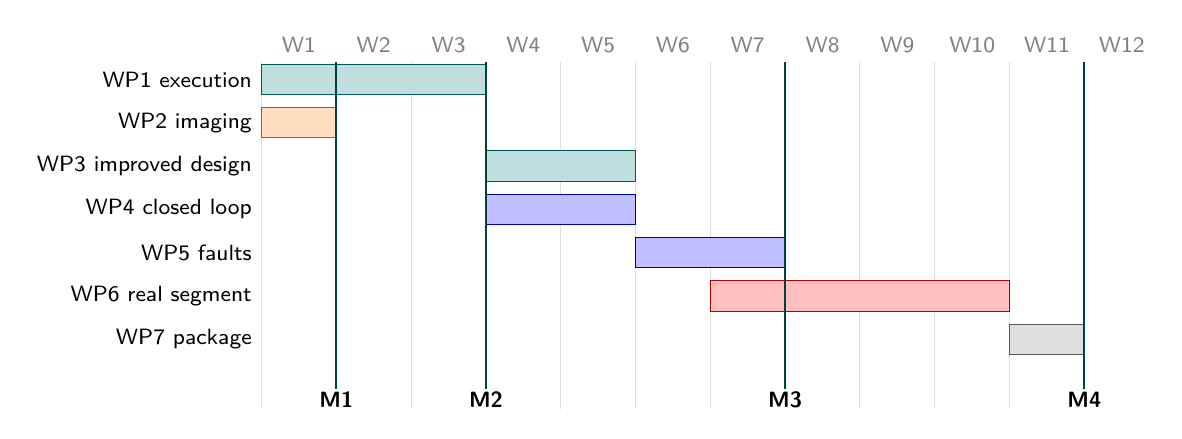
\begin{tikzpicture}[x=0.95cm, y=0.55cm, font=\footnotesize\sffamily]
\foreach \w in {0,...,11} {\draw[gray!25] (\w,0.4) -- (\w,-7.6); \node[gray] at (\w+0.5,0.8) {W\the\numexpr\w+1\relax};}
\def\bar#1#2#3#4{\fill[#4!25] (#2,-#1+0.35) rectangle (#3,-#1-0.35); \draw[#4!70!black] (#2,-#1+0.35) rectangle (#3,-#1-0.35);}
\bar{0}{0}{3}{teal}\node[anchor=east] at (0,0) {WP1 execution};
\bar{1}{0}{1}{orange}\node[anchor=east] at (0,-1) {WP2 imaging};
\bar{2}{3}{5}{teal}\node[anchor=east] at (0,-2) {WP3 improved design};
\bar{3}{3}{5}{blue}\node[anchor=east] at (0,-3) {WP4 closed loop};
\bar{4}{5}{7}{blue}\node[anchor=east] at (0,-4) {WP5 faults};
\bar{5}{6}{10}{red}\node[anchor=east] at (0,-5) {WP6 real segment};
\bar{6}{10}{11}{gray}\node[anchor=east] at (0,-6) {WP7 package};
\foreach \x/\m in {1/M1,3/M2,7/M3,11/M4} {\draw[thick,teal!50!black] (\x,0.4) -- (\x,-7.2); \node[fill=white,inner sep=1pt] at (\x,-7.4) {\textbf{\m}};}
\end{tikzpicture}\end{center}
\begin{description}[style=nextline]
\item[M1 (week 1)] the robot's images of every arm valid with registration.
\item[M2 (week 3)] the current design executed end to end in the twin by the generated plans; O2 checked on the executed
trail, not only on the plan.
\item[M3 (week 7)] the improved design carried through the proof; fault campaign with experiment-level consequences;
the closed loop proposes the next experiment.
\item[M4 (week 11)] one real segment against the twin's prediction; demonstrator package.
\end{description}

\begin{table}[htbp]\centering\footnotesize\caption{Acceptance criteria of D1.}
\begin{tabularx}{\linewidth}{@{}p{4.2cm}X@{}}\toprule criterion & measure \\\midrule
Faithful execution & the executed trail satisfies every culture-level obligation (O2 on the trail) in every nominal run \\
Valid observation & share of robot images valid; field offset from the culture within the 4$\times$ field \\
Proof coverage & refinement theorem regenerated and holding for both designs \\
Robustness & every injected fault ends in a handler with its guarantee; the conclusions it invalidates are named \\
Closed loop & belief updated from the robot's images; next experiment proposed with its expected gain \\
Twin vs real & the real segment's duration and outcome against the twin's prediction (target set after the first measurement) \\\bottomrule\end{tabularx}\end{table}

\begin{table}[htbp]\centering\footnotesize\caption{Risks.}
\begin{tabularx}{\linewidth}{@{}p{4.2cm}X@{}}\toprule risk & mitigation \\\midrule
No CRAM runtime on this machine & use PyCRAM or the kernel's Isaac backend as the executive for D1; keep the CRAM/RPL output as the reference \\
One 8 GB GPU: concurrent Isaac jobs crash it & serialize GPU jobs in the build pipeline \\
Integration of Giskard with the twin & start with R01 legs; fall back to the twin's own planners for R02 \\
Real hardware availability & decide the platform early (week 2); the twin demonstrator stands on its own \\
Biology realism & keep the surrogate labelled; invite scientists to pose the question for a later demonstrator \\\bottomrule\end{tabularx}\end{table}


\paragraph{Decisions needed} (1) the executive for D1: Lisp CRAM, PyCRAM, or the kernel's Isaac backend; (2) the
real-hardware segment and platform; (3) the audience and date of the first showing.

\begin{thebibliography}{9}\small
\bibitem{verid} P.~Rao, P.~Sirkovic, A.~Pawlosky. Grounding AI agents in biological reality: building blocks for
autonomous wet labs. Google Research blog, 16 Oct 2026.
\bibitem{safesdl} Z.~Zhang et al. Safe-SDL: establishing safety boundaries and control mechanisms for AI-driven
self-driving laboratories. arXiv:2602.15061, 2026.
\bibitem{baker2016} M.~Baker. 1,500 scientists lift the lid on reproducibility. Nature 533:452--454, 2016.
\bibitem{lapp} A.~Wolf et al. The Laboratory Automation Plug and Play (LAPP) framework, part three. ISPE iSpeak, 2026.
\bibitem{tracebot} TraceBot: traceable robotic handling of sterile medical products. EU H2020, grant 101017089, 2021--2025.
\end{thebibliography}
\end{document}
